%%
%%  Example paper
%%
%%

%%%%%%%%%%%%%%%%%% Usenix style %%%%%%%%%%%%%%%%%%%%%%%%%%%%%%%%%
\documentclass[10pt,twocolumn,a4paper]{article}
\usepackage{styles/usenix-style}

\author{Jakob Schmid}

%%%%%%%%%%%%%%%%%% Document %%%%%%%%%%%%%%%%%%%%%%%%%%%%%%%%%%%%%%%%%%%
% TODO: Change draft to final before submitting final version.
\usepackage[draft]{styles/ka-style}
\usepackage{cite,xspace,ifthen,graphicx,listings,url}

\usepackage[
   pdfauthor={Author},
   pdftitle={A Paper Template},
   pdfsubject={Paper Template},
   pdfkeywords={Papers, Templates}
]{hyperref}

\begin{document}

\title{Unikernel Linux (UKL)}

\newcommand{\todo}[1]{{\texttt{[#1]}}}
\newcommand{\code}[1]{{\tt \small{#1}}}
\newcommand{\refsec}[1]{{§ \ref{#1}}}

\maketitle
%\draftfooter

\begin{abstract}
  This report discusses Unikernel Linux (UKL), an approach to introduce a
  unikernel target into the Linux kernel.
  The specialized demand of cloud services has recently given rise
  to a resurgence of library operating systems in the form of unikernels.
  The authors of the UKL paper want to show that the Linux kernel can be
  modified to include the benefits of unikernels, while maintaining the
  ecosystem of applications and maintainers of Linux.
\end{abstract}

\section{Introduction}\label{sec:introduction}
  Modern cloud services are often highly specialised, to the point of a microservice, 
  where an applications is split up into a collection of loosely coupled services,
  that communicate through lightweight protocols and each only fullfill a single purpose.
  These services share a few key demands. They need to be able to communicate 
  efficiently with each other. Since they need to communicate with other services,
  they are exposed to the internet to some degree and thus should be as secure as possible.
  Due to the single purpose nature of the microservices they often execute as a single process.
  Lastly the image the service is executed with and the memory usage should be as small as possible.
  The services are often executed in a virtual machine on rented hardware, so lower requirements
  in memory and storage can improve the profitability of a service.
  These demands have caused a resurgence of research exploring the concept of 
  a library operating system (libOS) and the emergence of unikernels. 

  In a libOS a target application is linked with a set of
  libraries that provide all the services a regular OS would usually provide.
  The resulting executable can then be deployed directly to hardware.
  In 2013 the term \textit{unikernel} was first introduced for libOSs
  for cloud services and deployment to virtual hardware \cite{madhavapeddy13}.

  Since then multiple unikernels have been created. Some are written from scratch like
  ClickOS \cite{martins2014} and Unikraft \cite{kuenzer21}.
  Others borrow code from an existing OS like Drawbridge \cite{porter11} 
  that uses code from Windows.

  UKL uses the Linux kernel as a base but tries to keep the changes minimal
  so that UKL can be maintained with the (general purpose) Linux kernel.
  

\section{Background}\label{sec:background}
  \subsection{General-purpose monolithic operating systems}
    In a general-purpose monolithic operating system, such as Linux and Windows,
    the operating system (OS) defines an interface to use the physical resources
    of the system. 
    This interface hides details about the physical resources behind
    high-level abstractions like processes, files, addresss spaces 
    and interprocess communication.
    Applications running on the system use this interface and its abstractions
    to utilize the physical resources of the system.
    The implementation of the abstractions must be general to allow the execution 
    of very different applications.
    The OS also ensures that different applications can execute concurrently, 
    without interfering with each other. 
    Virtual address spaces are used to allow for simultanious usage of physical memory.
    Access to other resources, such as files and network communication, is controlled
    by the OS.
    This protection requires that applications must not be able
    to modify or replace the implementation of the abstractions supplied by the OS.

  \subsection{Library operating systems}\label{sec:libOS}
    One of the problems of the fixed abstractions for system resources in general-purpose OSs
    is that it denies applications the advantage of domain-specific optimizations.
    For example in 1994 Cao et al. \cite{cao94} showed that application-controlled file caching
    can reduce application running time by 45\%.

    In the mid 1990s the libOS was proposed as a different OS architecture
    where the application can control the hardware abstractions, instead of the OS \cite{engler95}.
    In a libOS the hardware resources are not controlled and protected by a kernel.
    Instead a set of application-level libraries implement the mechanisms to drive hardware,
    communicate over the network and all other functionality a general-purpose 
    operating system would provide for an application.
    Further a set of policies are used to enforce access control and isolation in the
    application layer \cite{madhavapeddy13-2}.
    
    The libOS architecture allows applications to access hardware resources directly
    thus eliminating the need for repeated privilege transitions to move data
    between kernel and user space.
    In addition applications can now choose a library to drive the hardware that is
    taylored to the needs of that specific application, thus improving performance.
    This architecture also makes the performance more predictable.
    In a monolithic OS the kernel might schedule a different process after a
    context switch or do signal handling before handing control back to the application.

    Compiling an application with only the libraries the application requires
    can significantly reduce the amount of code involved.
    This reduction in code can not only lead to a reduction in image size, 
    but can also decrease the chance of the code containing a 
    security vulnerability \cite{madhavapeddy13}.

    The libOS architecture has two major disadvantages:   
    One, it is hard to achieve strong resource isolation because not all
    usage of hardware resources has to go through one abstraction supplied by
    a kernel like in a monolithic OS.
    Two, device drivers have to be rewritten to work as a library rather than
    for example a kernel module.
    This implementation effort has caused problems with hardware compatability
    for libOS projects and thus mostly limited their relevance to the
    research domain \cite{madhavapeddy13}.

  \subsection{Unikernels}
    OS virtualisation can overcome both of the major disadvantages of libOSs
    mentioned in \refsec{sec:libOS}.
    The lack of resource isolation between applications can be avoided by
    dedicating a seperate virtual machine (VM) to each application.
    This delegates resource isolation from the OS level to the hypervisor.
    The hypervisor offers a much simpler, less fine grained interface than
    a conventional OS, consisting of virtual CPUs and memory pages, 
    rather than the process-oriented approach in conventional OSs \cite{madhavapeddy13-2}.
    Dedicating a seperate VM to each application also leaves more room
    to specialize the VM to its particular purpose.
    The problem of hardware compatability of libOSs can also be overcome
    with virtualization. The libOS only has to implement drivers for
    the virtual hardware devices offered by the hypervisor.
    The hypervisor is then responsibel for driving the ever changing physical
    hardware.

    Madhavapeddy et al. introduced the term unikernel in a paper 
    published in 2013 \cite{madhavapeddy13}.
    Here unikernels are described as an approach to deploy cloud services
    using specialised single-purpose libOS VMs running directly 
    on the hypervisor \cite{madhavapeddy13}.

    Despite the benefits of the unikernel approach, they have not yet been widely adopted
    outside of the research and experimental domain.
    This could be attributed to the engeneering burden of porting existing software
    to an environment with no or only partial support for legacy software interfaces \cite{raza19}.
    
    \subsubsection{Performance and size}
      Deploying a service using a unikernel can offer significant
      performance advantages.
      Typical optimisations other than using libraries specialised for the given
      application inlcude avoiding ring transition overheads \cite{maeda2003},
      leveraging the single address space to pass pointers rather than copying data \cite {schatzberg16},
      deferring preemption in latency sensitive routines,
      exploiting application knowledge to remove code that is never executed \cite{madhavapeddy13},
      and cross layer optimization between kernel and application code \cite{raza19}.

      Memcached running on a unikernel TCP/IP stack
      demonstrated a 200\% throughput improvement compared to Linux \cite{schatzberg16},
      unikernels deployed within a microVM have shown six to ten times shorter
      boot times over containers \cite{koller17} and a micropython unikernel reached an image
      size of 1MB while requireing 8MB of memory to run \cite{manco17}.

    \subsubsection{Thread model}\label{sec:thread-model}
      Unikernels are per definition concerned with applications that provide network
      facing services. 
      The focus on virtual hardware and deployment to a hypervisor
      often implies usage in a multi-tenant datacenter.
      Here the provider of the datacenter is trusted not to be malisious.
      Other tenants and internet-connected hosts in general are seen as 
      a potential attacker.
      Internally the hypervisor is used as the sole unit of isolation, 
      rather than adopting a multi-user access control model as most general purpose OSs do.
      External entities the unikernel communicates with are trusted through
      protocol libraries such as SSL or SSH \cite{madhavapeddy13}.

    \subsubsection{Security}
      A problem with images based on a general purpose OSs is that misconfiguration can
      leave unneeded or unnecessary services running. 
      These services can significantly increase the remote attack surface.
      When creating an appliance using the unikernel approach only the libraries
      needed by the particular application are included in the final image.
      Thus no unnecessary services are included in the final image.
      Further this can also drastically deacrease the amount of code included and thus the chance
      for a vulnerability in the code.
      
      About 70\% of vulnerabilities in Windows, a general purpose OS written in C/C++,
      that Microsoft assigns a CVE each year are memory safety issues \cite{msrc-19-07}.
      Unikernels written in high level programming languages with a strong type system 
      can use high level language features for memory management to negate a large
      portion of these vulnerabilities \cite{madhavapeddy13, lankes19}.
      MirageOS \cite{madhavapeddy13}, a unikernel written in OCaml, can be sealed \cite{hunt07} at runtime,
      thus preventing any code not present at compile time from being executed.
      MirageOS further implements compile-time address space randomization to defend against
      return-oriented programming attacks and save on runtime complexity.
      This is justified by the fact that for unikernels reconfiguring the appliance 
      means recompiling it, potentially for every deployment \cite{madhavapeddy13}.

      Another aspect of unikernel security is that the chance for a common exploit is lower.
      An exploit found in the linux kernel can potentially affect all machines running Linux
      due to them sharing a vast majority of their code.
      Each unikernel however is specialized to suit the needs of only one application thus
      sharing less code with other appliances using the same unikernel.
      The smaller amount of shared code decreases the probability of an exploit being applicable
      to many unikernel appliances.

    \subsubsection{Categorisation of unikernels}\label{sec:categories-of-unikernels}
      \textit{Clean slate} unikernels are written from scratch.
      Here the unikernel designers have full control over the language
      and the methodology used \cite{raza19}.
      Thus the unikernel can be specialised to an abitrary degree to service the needs
      of a particular class of applications.
      The interface available to the application can also be choosen freely.

      In \textit{strip down} unikernels an existing kernel code base is forked
      and all functionality not needed for the unikernel is removed.
      The interfaces and general purpose libraries can be perserved to some degree
      to make porting of existing applications written for the original kernel
      over to the unikernel easier. 
      This generality however comes at the cost of loosing room for specialisation,
      efficient pathways and fine-tuned implementation.
      The creation of an out-of-tree fork of an existing OS comes with the burden of
      having to manually port updates from the original OS to the unikernel at regular intervals
      in order to keep the support for existing applications \cite{raza19}.
      
\section{Related Work}\label{sec:relwork} 
  \subsection{Kernel Mode Linux}
    Kernel Mode Linux (KML) is an operating system that allows
    execution of user processes in kernel mode on IA-32 CPUs.
    Based on the observation that system calls can be 36 times slower
    than function calls \cite{maeda2003} KML allows applications to execute in
    kernel mode, thus allowing the usage of function calls instead of system calls.
    An application executing in kernel mode would be capable of accessing kernel
    memory and compromise the integrity of the system.
    To prevent this KML uses TALx86 a typed assembly language.
    The authors of KML prove that using the typed assembly language guarantees the 
    same amount of safety as using traditional hardware-based protection of the kernel \cite{maeda2003}.
    In order to benefit from that safety applications for KML have to be written in
    either TALx86 or Popcorn, a safe dialect of the C programming language.
    Here instead of using system calls the programmer can now use function calls for improved performance.

    Existing applications can also be executed in kernel mode but do not come with
    the mentioned safety guarantees.
    This is made possible by adding a new branch to the system call invocaion multiplexer
    that invokes system calls with direct function calls \cite{maeda2003}.
    The multiplexer executes additional instructions to invoke the system call however, 
    so this mechanism is not optimal but still sudiciently fast compared to regular system call
    invokation.

  \subsection{Lupine Linux}
    Lupine Linux tries to achive unikernel-like performance and benefits in Linux.
    This is achieved through, one, specialization by using the existing Kconfig 
    configuration mechanism of the Linux kernel, 
    and two, system call overhead elimination using KML.

    For specialisation only 283 of the 15,953 Kconfig configuration options where
    selected as a base configuration \cite{kuo20}.
    With a total of 19 different additional options the top 20 most popular cloud applications,
    determined through Dockerhub download numbers, could all be succesfully executed.

    In benchmarks Lupine Linux outperformed AWS Firecracker's MicroVM, a lightweight 
    kernel image for general cloud application. 
    Lupine Linux also outperformed OSv \cite{osv}, 
    one the POSIX-like unikernels used for reference \cite{kuo20}.

\section{Approach}\label{sec:approach}
  \subsection{Goals}\label{sec:goals}
    The goal of UKL is similar to that of Lupine Linux, in that it aims
    to bring the benefits promised by unikernels to the Linux kernel.
    UKL tries to achieve this while one, maintaining the rich support for hardware devices of Linux.
    Two, UKL aims at retaining the compatability with existing legacy software for the Linux kernel.
    And three, UKL want to preserve the ecosystem of tools for testing and debugging the kernel.
    Preserving this ecosystem and keeping the changes to the Linux kernel als minimal as possible
    would also increase the chance of UKL to be accepted by Linux community.
    As mentioned in \refsec{sec:categories-of-unikernels}, manually porting updates from
    the Linux kernel to UKL would require a continious effort.
    To get around this the authors of UKL aim to have UKL included in the upstream Linux kernel
    \cite{ukl-redhat-post}.

    In a previous paper \cite{raza19} the authors of the UKL paper \cite{raza23}
    observed that applications that require high-performance IO use frameworks
    to bypass the kernel and gain unimpeded access to hardware devices \cite{raza19}.
    This combined with the promised benefits of unikernels creates a need to act
    for the Linux community in order to stay dominant for cloud computing, according to the authors.
    The goal of UKL is to provide the proof that Linux can be adapted to suit the new demands of
    cloud computing and retain its dominant position in the world of modern cloud computing.

  \subsection{Incremental approach}
    UKL follows a so-called incremental approach. 
    Each increment is less general purpose but can bring performance benefits.
    The lowest increment is the base model which perserves almost all the 
    invariants and assumptions of applications written for Linux.
    The performance benefit of the base model is negligible.
    After the application runs on the base model the developer can choose to try different
    configuration options for a higher performance improvement.
    These configuration options might not work with every application, but are easy to try out
    with just a recompilation.
    For more perfomance improvement the developer can choose to modify the application, exploiting the
    knowledge about the application to invoke kernel functionality directly.

  \subsection{Base model}
    In the base model an application is compiled and statically linked with both 
    the UKL kernel and a modified version of glibc to create a bootable image.
    When executed this image will have a UKL-optimised process executing the supplied 
    application in kernel-mode.
    Different to most other unikernels, in UKL regular user-level processes are still possible.
    This is crucial to support debugging and testig tools and initialization scripts needed by
    some applications (see \refsec{sec:goals}).
    User-level processes are however not protected from the UKL-optimised one.
    This is in line with the security model of unikernels where all work that has to 
    be protected is isolated through the hypervisor (\refsec{sec:thread-model}).

    \subsubsection{Address space layout}
      Most unikernels have a single address space due to their single process nature.
      UKL differs in that it retains the split of the virtual address space into kernel and user-space.
      For the UKL-optimised process the code and data segments move to kernel space because
      the application and the kernel are compiled and linked together.
      All other memory regions of the UKL-optimised process remain in user-space.

      This layout could be problematic for applications with large initialized data sections
      that are pinned in UKL due to being in kernel-space.
      According to the authors of the UKL-paper changing this layout would have required changes
      to the Linux kernel that may be difficult to upstream (see \refsec{sec:goals}).

      The virtual address space of regular user-level processes remains unchanged from
      the classic Linux virtual address space layout.


\section{Conclusion}\label{sec:conclusion}






\begin{figure}[htbp]
  \centering
  \fbox{\parbox{.8\columnwidth}{
      Here you can include a sample figure.  Use something like
      \begin{center}
        \code{$\backslash$includegraphics[scale=.8]\{template\}}
      \end{center}
      to include an encapsulated postscript figure.  The \emph{scale}
      argument can be used for scaling the picture, although it
      may scale the font incorrectly.
    }}
  \caption{Sample Figure}
  \label{fig:sample}
\end{figure}


\lstset{language=C, basicstyle=\ttfamily,
        string=[b]', showspaces=false, showtabs=false,
        caption={A sample code snippet}, captionpos=b}
\begin{lstlisting}
/* code snippet  */
while (!sleep)
	sleep++;
\end{lstlisting}

\begin{figure}[hbt]
\centering
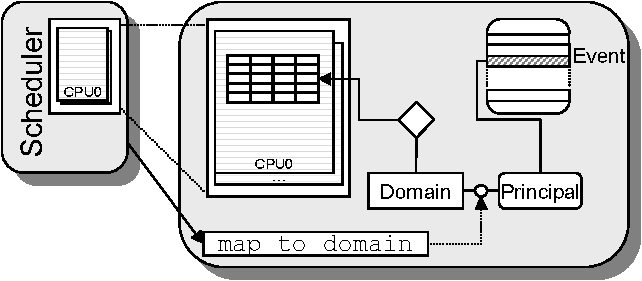
\includegraphics[scale=.7,clip]{fig/template}
\caption{Sample figure automatically from Windows prn.\label{plot:fig}}
\end{figure}


Works \cite{xen03virtualization} and \cite{pratt2005xaa} are relevant but
different.


\bibliographystyle{plain}
\bibliography{template}
%\footnotesize
\end{document}
